\section{Testing}
\subsection{Analisi statica}
Per l'analisi statica del codice Java è stato utilizzato il tool STAN4J, integrato nel IDE Eclipse. Il report è riportato a fine capitolo.

\subsection{Analisi dinamica}
Nell'iterazione 3 si sono testate tutte le API Rest implementate, utlizzando Postman (\Fig \ref{fig:RisultatiTestAPIIT3}). In particolare si sono testate le seguenti funzionalità:

\begin{itemize}
	\item AreaController:
	\begin{itemize}
		\item Visualizzazione degli ultimi dati meteo scaricati di un'area, il cui id è specificato nel path della richiesta;
		\item Visualizzazione del più recente allarme relativo a nebbia o brina associato all'area il cui id è specificato nel path della richiesta;
		\item Visualizzazione del più recente allarme relativo a maltempo associato all'area il cui id è specificato nel path della richiesta;
	\end{itemize}

	\begin{figure}[h!]
		\centering
		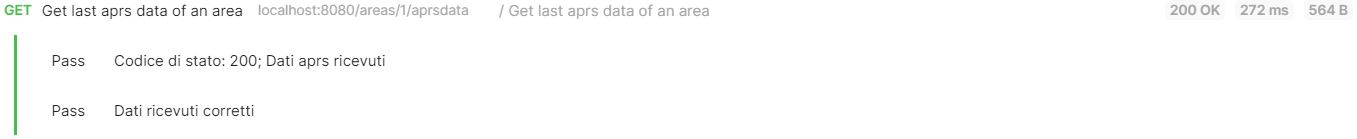
\includegraphics[width=1\linewidth]{./Iterazione 3/ImageFiles/TestGetAprsData}
		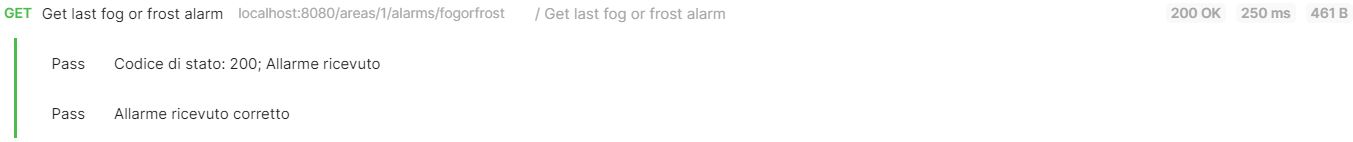
\includegraphics[width=1\linewidth]{./Iterazione 3/ImageFiles/TestGetFrostOrFogAlarm}
		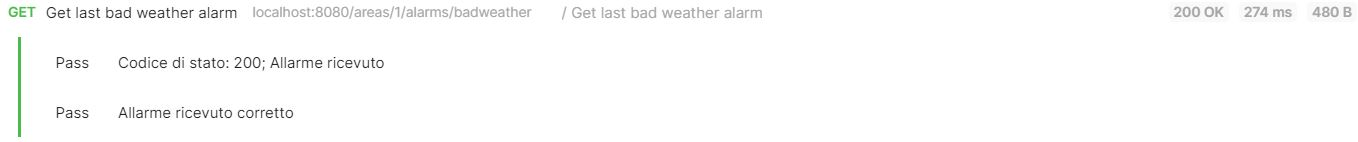
\includegraphics[width=1\linewidth]{./Iterazione 3/ImageFiles/TestGetBadWeatherAlarm}		
		\caption{Risultati test API su Postman.}
		\label{fig:RisultatiTestAPIIT3}
	\end{figure}

\clearpage

	\item UserController:
	\begin{itemize}
		\item Visualizzazione dell'ultima posizione disponibile di un utente attivo;
		\item Visualizzazione dell'ultima posizione disponibile di un utente inattivo;
		\item Inserimento della posizione di un utente;
	\end{itemize}
	\begin{figure}[h!]
		\centering
		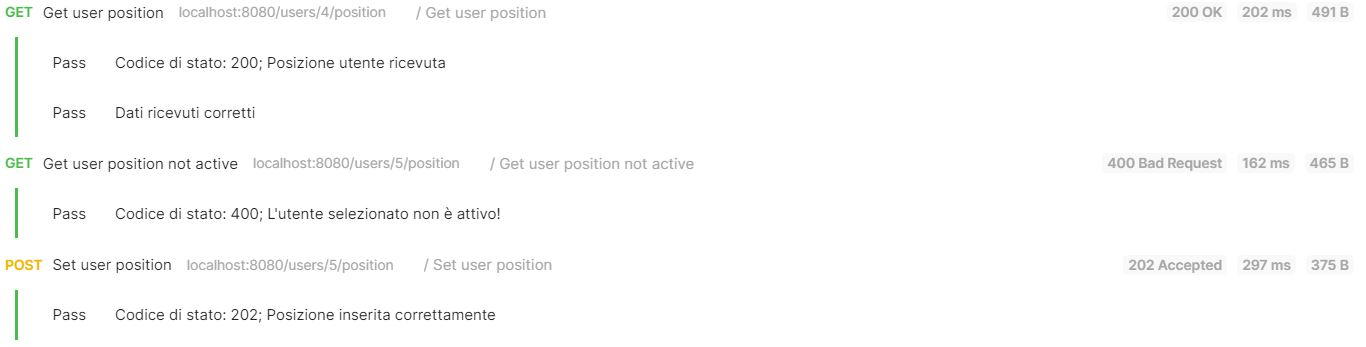
\includegraphics[width=1\linewidth]{./Iterazione 3/ImageFiles/TestUserController}
		\caption{Risultati test API su Postman.}
		\label{fig:RisultatiTestAPIIT3_2}
	\end{figure}
\end{itemize}

\clearpage

\subsection{Unit Test}
\subsubsection{LvsEmergency Server}
In questa iterazione è stata testata la funzione \texttt{findFirstByAprsDataIdNameOrderByAprsDataIdTimeDesc(String name)} che recupera i dati più recenti relativi alla stazione APRS, il cui \texttt{name} è specificato nel parametro. Di seguito è riportato il codice del test.

\lstinputlisting[language=Java]{./Iterazione 3/OtherFiles/AprsDataRepositoryTest.java}

Il risultato del test con JUnit ha confermato il corretto funzionamento della funzione.

\begin{figure}[h!]
	\centering
	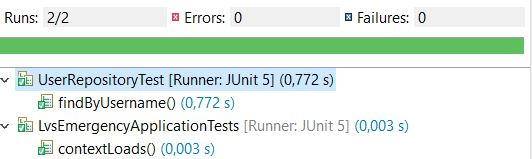
\includegraphics[width=0.6\linewidth]{./Iterazione 3/ImageFiles/TestJUnit}
	\caption{Risultato test con JUnit.}
	\label{fig:RisultatiTestJunitIT3}
\end{figure}

\clearpage

\subsubsection{Client App}
Lato client è stata testata la corretta creazione delle classi aggiunte nell'iterazione 3, \texttt{AprsData} e \texttt{Alarm} a partire da una stringa JSON. Di seguito è riportato il codice del test: 

\lstinputlisting[language=C++]{./Iterazione 3/OtherFiles/testcpp.cpp}

Il risultato dei test ha confermato il corretto funzionamento delle nuove funzioni e di quelle precedenti. 

\begin{figure}[h!]
	\centering
	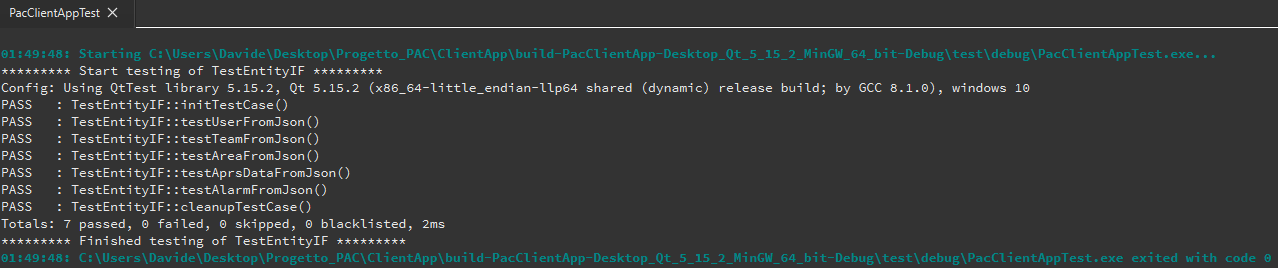
\includegraphics[width=1\linewidth]{./Iterazione 3/ImageFiles/testQt}
	\caption{Risultato test con Qt Test.}
	\label{fig:RisultatiTestQtIT3}
\end{figure}


Inoltre, è stata testata la corretta creazione della classe \texttt{Position} a partire da una stringa JSON. Di seguito è riportato il codice del test: 

\lstinputlisting[language=C++]{./Iterazione 3/OtherFiles/testcpp2.cpp}

Il risultato dei test ha confermato il corretto funzionamento delle nuove funzioni e di quelle precedenti. 

\begin{figure}[h!]
	\centering
	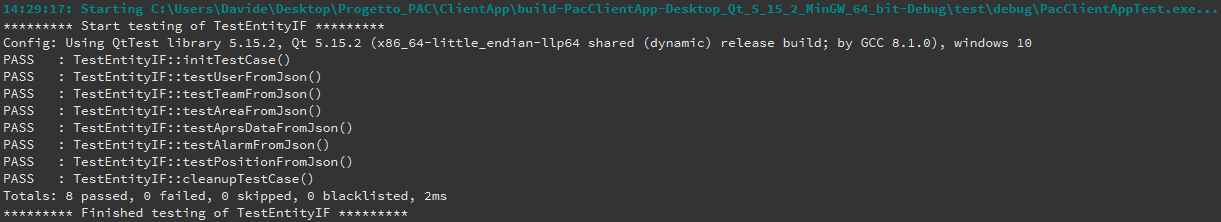
\includegraphics[width=1\linewidth]{./Iterazione 3/ImageFiles/testcpp2}
	\caption{Risultato test con Qt Test.}
	\label{fig:RisultatiTestQtIT3.2}
\end{figure}

\subsection{Test Data Analyzer}
Sono stati eseguiti anche dei test di unità sull'algoritmo. Nella figura \ref{fig:test_result_alg} sono riportati i risultati effettuati grazie al modulo di Python \texttt{unittest}. Si è testato la generazione dei seguenti allarmi:
\begin{itemize}
	\item allarme \textit{RED} per maltempo e allarme \textit{RED} per nebbia;
	\item allarme \textit{NONE} per maltempo e allarme \textit{RED} per brina;
	\item allarme \textit{NONE} per maltempo e allarme \textit{NONE} per nebbia;
	\item allarme \textit{NONE} per maltempo e allarme \textit{WHITE} per nebbia;
	\item allarme \textit{NONE} per maltempo e allarme \textit{GREEN} per nebbia.
\end{itemize}

\begin{figure}[h!]
	\centering
	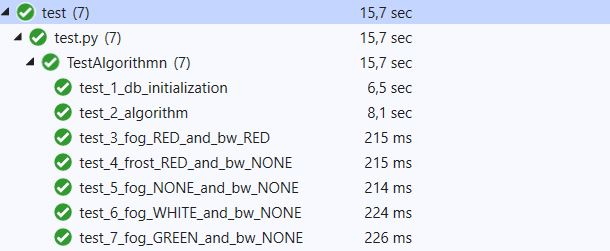
\includegraphics[width=1\linewidth]{./Iterazione 3/ImageFiles/TestResultAlgorithm}
	\caption{Risultati test algoritmo (interfaccia di Visual Studio).}
	\label{fig:test_result_alg}
\end{figure}

Di seguito è riportato il codice python relativo alla classe che implementa i test. Inizialmente, viene popolato un database di test con i dati caricati da dei file \textit{csv}. All'interno dei file è specificato il nome di una stazione APRS fittizia e i relativi dati di test di temperatura, umidità, pressione e data di acquisizione. Ogni test è associato a una diversa area.  Se le operazioni di caricamento terminano correttamente, viene lanciata l'esecuzione dell'algoritmo. Se non si verificano eccezione, vengono poi controllati gli allarmi inseriti dall'algoritmo: se corrispondono agli allarmi attesi, il test è superato.

\begingroup
\UseRawInputEncoding
\lstinputlisting[language=python]{./Iterazione 3/OtherFiles/test_algorithm_script.py}
\endgroup

Inoltre, si riporta un esempio di allerta nebbia di tipo \textit{RED} generata dall'algoritmo il 6 febbraio 2022 (\Fig\ref{fig:test_previsione_alg}) sulla stazione meteorologica situata nei pressi della località di Ospitaletto (BS). Si è potuto verificare che questa allerta rispecchiasse veramente la situazione meteo attuale. Infatti, le previsioni meteorologiche attuali fornite da Google indicavano la presenza di nebbia (\Fig\ref{fig:test_previsione_google}).

\begin{figure}[h!]
	\centering
	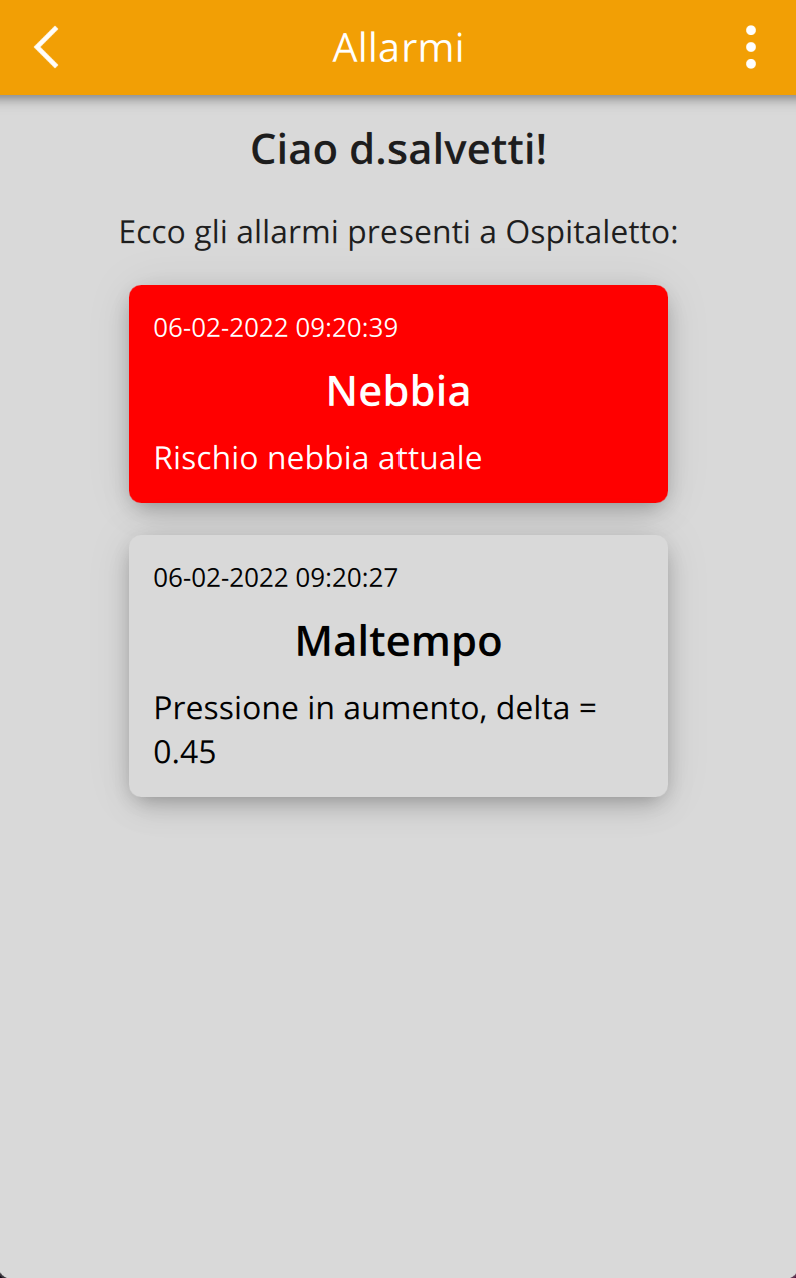
\includegraphics[width=0.3\linewidth]{./Iterazione 3/ImageFiles/testAppRedFog}
	\caption{Allarme nebbia attuale a Ospitaletto (BS) domenica 06/02/22 alle ore 9:20.}
	\label{fig:test_previsione_alg}
\end{figure}

\begin{figure}[h!]
	\centering
	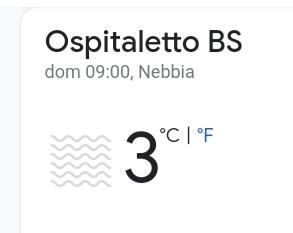
\includegraphics[width=0.2\linewidth]{./Iterazione 3/ImageFiles/Nebbia Ospitaletto Google}
	\caption{Meteo attuale fornito da Google a Ospitaletto (BS) domenica 06/02/22 alle ore 9:20.}
	\label{fig:test_previsione_google}
\end{figure}

\clearpage

\section{Documentazione API}

In questa sezione viene mostrata la documentazione relativa ad alcune API implementate nell'iterazione 3. \`E possibile visualizzare una collezione (creata con Postman) di tutte le API realizzate e testate sulla repository GitHub. In particolare, si riportano di seguito le più significative:
\begin{itemize}
	\item API per la visualizzazione degli ultimi dati meteorologici raccolti dalla stazione APRS associata all'area, il cui id è specificato nel path della richiesta;
	\item API per la visualizzazione del più recente allarme di nebbia o brina generato nell'area di interesse;
	\item API per la visualizzazione del più recente allarme di maltempo generato nell'area di interesse;
	\item API per la visualizzazione dell'ultima posizione disponibile di un utente attivo;
	\item API per l'inserimento della posizione di un utente;
\end{itemize}

\begin{figure}[h!]
	\centering
	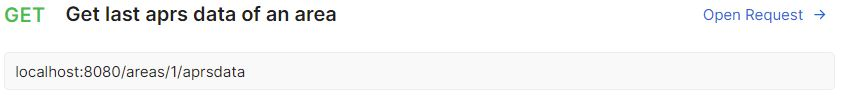
\includegraphics[width=1\linewidth]{./Iterazione 3/ImageFiles/GetAprsDataRequest}
	\lstinputlisting[language=json]{./Iterazione 3/OtherFiles/GetAprsDataResponse.json}
	\caption{Documentazione API Get Aprs data.}
	\label{fig:GetAprsDataAPI}
\end{figure}

\begin{figure}[h!]
	\centering
	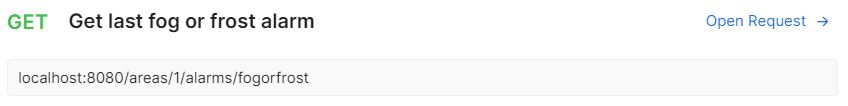
\includegraphics[width=1\linewidth]{./Iterazione 3/ImageFiles/GetFrostOrFogAlarmRequest}
	\lstinputlisting[language=json]{./Iterazione 3/OtherFiles/GetFrostOrFogAlarmResponse.json}
	\caption{Documentazione API Get fog or frost alarm.}
	\label{fig:GetFrostOrFogAlarm}
\end{figure}

\begin{figure}[h!]
	\centering
	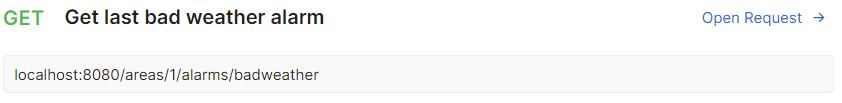
\includegraphics[width=1\linewidth]{./Iterazione 3/ImageFiles/GetBadWeatherAlarmRequest}
	\lstinputlisting[language=json]{./Iterazione 3/OtherFiles/GetBadWeatherAlarmResponse.json}
	\caption{Documentazione API Get bad weather alarm.}
	\label{fig:GetBadWeatherAlarm}
\end{figure}

\begin{figure}[h!]
	\centering
	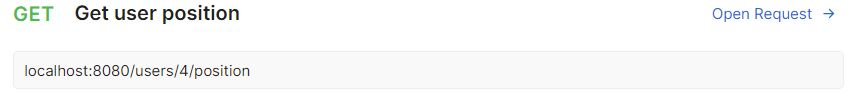
\includegraphics[width=1\linewidth]{./Iterazione 3/ImageFiles/GetUserPositionRequest}
	\lstinputlisting[language=json]{./Iterazione 3/OtherFiles/GetUserPositionResponse.json}
	\caption{Documentazione API Get user position.}
	\label{fig:GetUserPosition}
\end{figure}

\begin{figure}[h!]
	\centering
	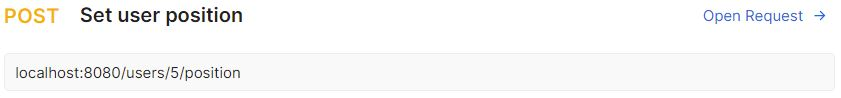
\includegraphics[width=1\linewidth]{./Iterazione 3/ImageFiles/SetUserPositionRequest}
	Body:
	\lstinputlisting[language=json]{./Iterazione 3/OtherFiles/SetUserPositionBody.json}
	Response:
	Position set correctly!
	\caption{Documentazione API Set user position.}
	\label{fig:SetUserPosition}
\end{figure}

\clearpage

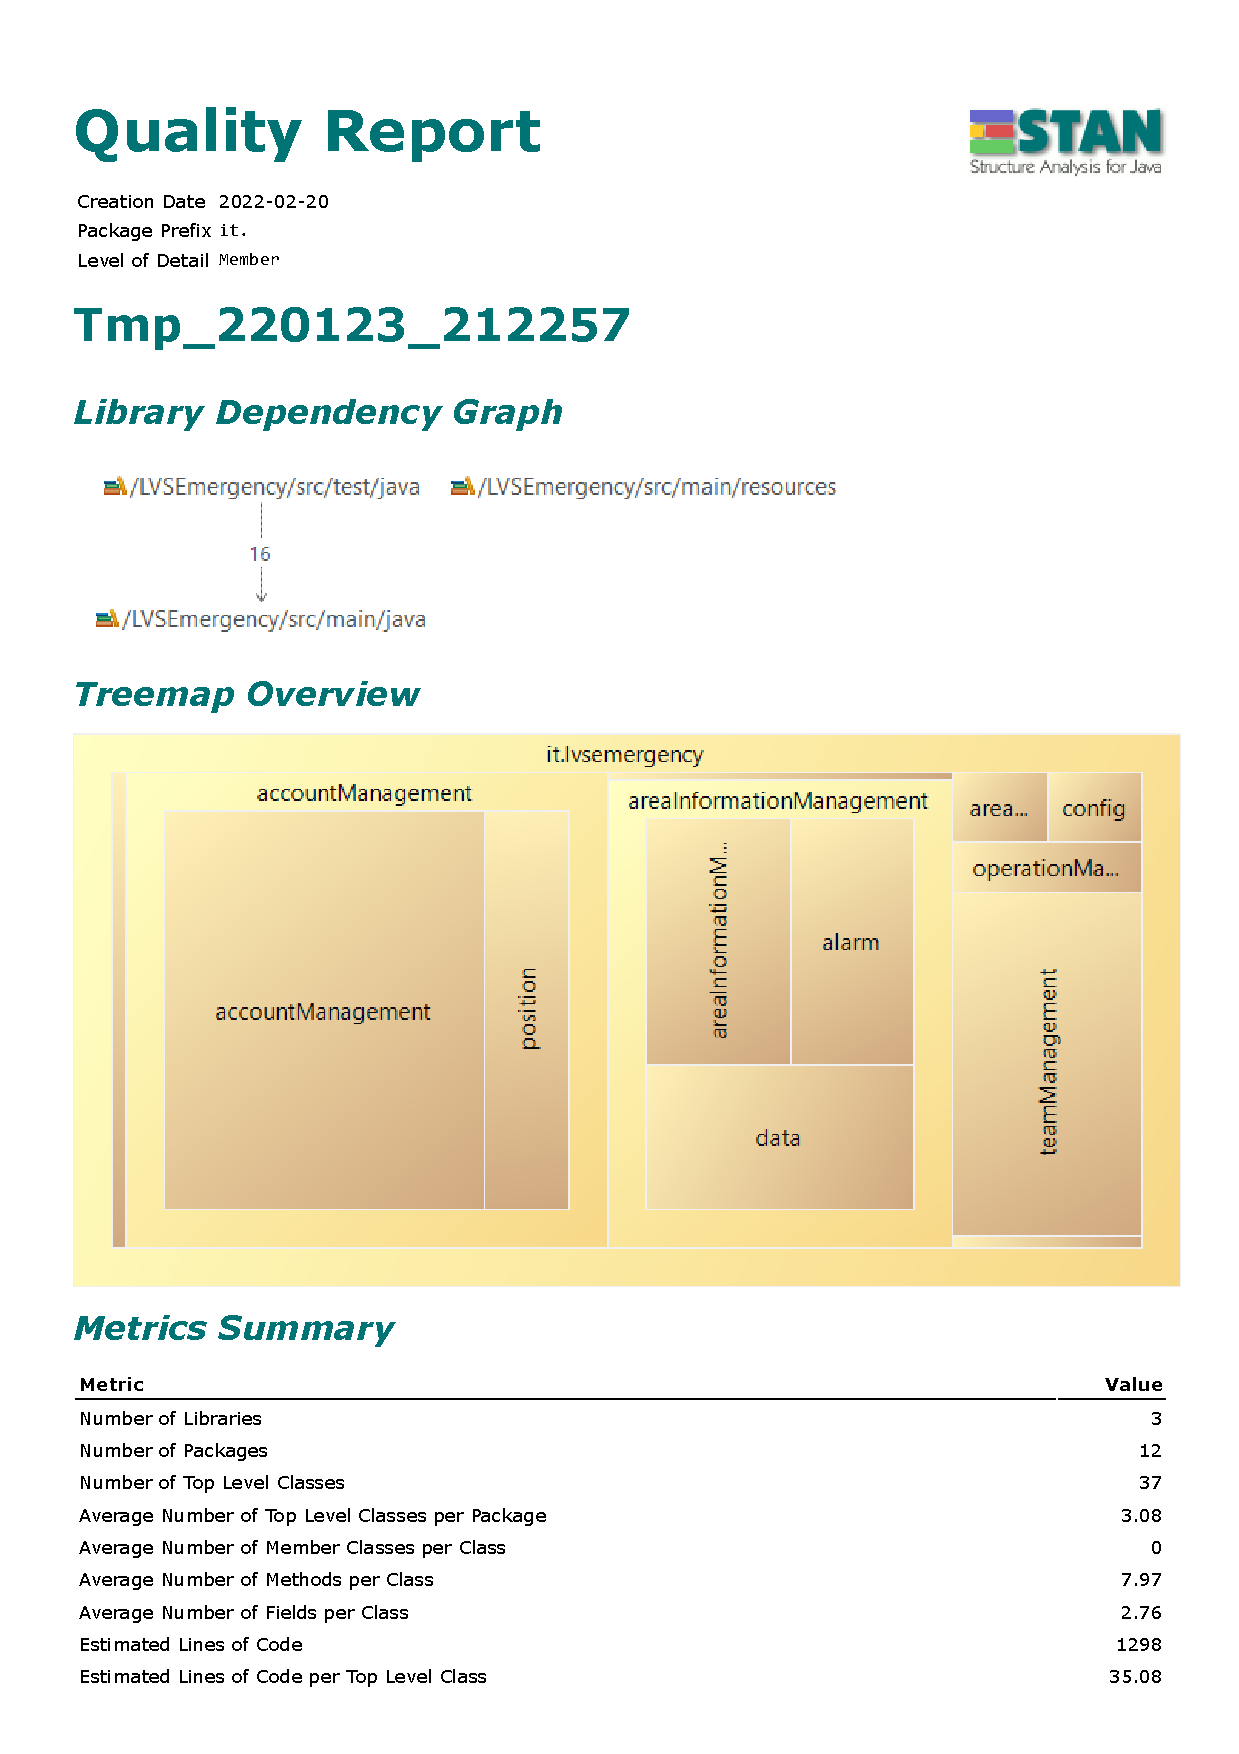
\includepdf[pages=-]{./Iterazione 3/OtherFiles/Report STAN4J/Quality Report}
